\section{Analisis Solusi}

\subsection{Ide Dasar}

Sebagaimana dijelaskan pada analisis masalah, kita harus mengatasi masalah \textit{read query} ketersediaan tiket serta \textit{throughput} dan \textit{flow control} pemesanan tiket. Berikut adalah ide dasar untuk menyelesaikannya:

\begin{enumerate}
  \item Permasalahan pada \textit{read query} dapat diatasi dengan memanfaatkan \textit{streaming database}, sehingga sistem menyediakan \textit{query} hasil agregasi yang diperbarui secara \textit{incremental} setiap kali ada perubahan. Pendekatan ini mengurangi proses agregasi yang dilakukan secara berulang-ulang, sehingga \textit{query} lebih efisien. Selain itu, pendekatan ini membagi tanggung jawab untuk operasi \textit{read} dari basis data utama.
  \item Terdapat dua opsi untuk meningkatkan \textit{throughput} pemesanan tiket, yaitu dengan melakukan \textit{row-level sharding} pada relasi tiket dan menggunakan \textit{extension} Citus yang memungkinkan adanya \textit{multiple writer}. Di sisi lain, menghilangkan basis data relasional sepenuhnya juga bisa menjadi opsi. Pendekatan \textit{database inside-out} yang memisahkan komponen \textit{storage}, \textit{query}, dan lain-lain dari basis data memungkinkan setiap komponen \textit{scale} secara terpisah dan mencapai \textit{scalability} yang lebih baik. Meskipun begitu, perlu desain khusus untuk menjamin tidak terjadi \textit{double booking} dan menjamin integritas \textit{transaction}.
  \item Untuk mengatur \textit{flow control}, pendekatan \textit{queue-based load leveling pattern} dapat digunakan dengan membuat operasi pemesanan asinkron dan membuat \textit{queue}. Dengan begini, sistem dapat memproses permintaan sesuai dengan kapasitas sistem dan stabilitas sistem dapat terjaga. Selain itu, sistem dapat menyimpan \textit{dirty/ uncommited data} tiket (tiket yang sedang dipesan, tetapi belum \textit{commited}). Dengan memanfaatkan data tersebut, sistem dapat menolak \textit{request} sehingga mencegah \textit{request} masuk sedari awal. 
\end{enumerate}

Secara umum, solusi yang dibahas mengikuti pola yang menyerupai pendekatan CQRS.

\subsection{Komponen Sistem \textit{Ticketing}}

Berdasarkan studi yang sudah dibahas sebelumnya dan berdasarkan fokus yang ingin dibahas pada penelitian ini, berikut adalah komponen sistem yang menjadi \textit{scope} dari penelitian ini:

\begin{enumerate}
  \item Layanan \textit{backend} utama yang memproses setiap permintaan yang berkaitan dengan pemesanan tiket.
  \item Layanan \textit{authentication}.
  \item Layanan \textit{payment gateway}. Layanan ini merupakan \textit{external service} dan cukup melakukan \textit{mocking service}.
  \item Selain itu, terdapat satu basis data utama sebagai \textit{single source of truth}.
\end{enumerate}

Daftar acara dan ketersediaan awal tiket merupakan data yang di-\textit{populate} dari awal, sehingga fitur manajemen acara dan tiket tidak diimplementasikan. Pembahasan lengkap sistem dibahas pada bagian lampiran.

\subsection{Arsitektur Solusi}

\subsubsection{Arsitektur Dasar}

Arsitektur ini akan menjadi \textit{baseline} atau referensi yang digunakan sebagai dasar perbandingan kinerja. Terdapat dua layanan eksternal, yaitu layanan pengguna dan layanan pembayaran. Selain itu, terdapat \textit{cluster} PostgreSQL dengan konfigurasi satu \textit{leader node} dan beberapa \textit{read replica}. Keberadaan \textit{read replica} memungkinkan peningkatan \textit{read throughput} untuk operasi \textit{query} ketersediaan. Meskipun begitu, tidak ada pengoptimalan untuk operasi pemesanan tiket.

\begin{figure}[ht]
  \centering
  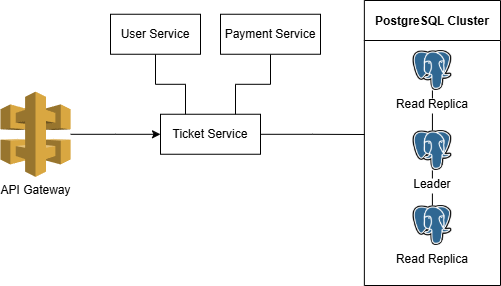
\includegraphics[width=0.8\textwidth]{resources/chapter-3/architecture-reference.png}
  \caption{\textit{Baseline Architecture}}
  \label{fig:baseline-architecture}
\end{figure}

Basis data merupakan komponen yang sulit di-\textit{scale} secara dinamis berdasarkan beban yang diterima. Pada konfigurasi ini, \textit{vertical scaling} merupakan satu-satunya opsi untuk meningkatkan \textit{throughput}. Meskipun begitu, layanan lain seperti \textit{ticketing service} dan layanan pengguna dapat dengan mudah di-\textit{scale} dengan menambah jumlah \textit{instance}.

\subsubsection{Arsitektur yang Mengoptimalkan PostgreSQL}

Arsitektur ini mengoptimalan sistem dengan pola CQRS. Tanggung jawab penanganan \textit{read query} dilimpahkan kepada RisingWave \textit{instance}. \textit{Streaming database} ini mengonsumsi \textit{CDC stream} dari \textit{PostgreSQL cluster}, melayani permintaan \textit{query} ketersediaan tiket, serta memperbaruinya secara \textit{incremental}. \textit{Cluster} PostgreSQL dengan \textit{extension} Citus memungkinkan penggunaan \textit{row-based sharding} dengan \textit{multiple writer} sehingga \textit{write throughput} dapat ditingkatkan. Selain itu, permintaan pemesanan tiket akan di-\textit{queue} terlebih dahulu lalu diproses secara bertahap. Redis digunakan untuk menyimpan \textit{dirty data} dari transaksi yang sudah \textit{commited} dan \textit{uncommited} sehingga dapat mencegah permintaan pemesanan masuk. Kedua pendekatan ini mengikuti pola \textit{queue-based load leveling}. Selain itu, pemodelan data yang digunakan untuk pemesanan tiket adalah berupa \textit{command}, yang merupakan varian dari \textit{event sourcing}.

\begin{figure}[ht]
  \centering
  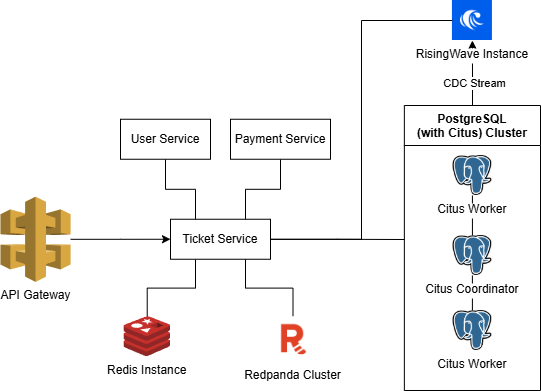
\includegraphics[width=0.8\textwidth]{resources/chapter-3/architecture-optimized.png}
  \caption{\textit{Optimized Architecture with PostgreSQL}}
  \label{fig:optimized-architecture}
\end{figure}

Basis data masih merupakan komponen yang sulit di-\textit{scale} secara dinamis. Meskipun begitu, penggunaan \textit{extension} Citus memungkinkan peningkatan \textit{write throughput} dengan \textit{scale out} dan tidak hanya dengan \textit{scale up}. \textit{Instance} Redpanda dapat dengan mudah dibuat \textit{cluster} dan \textit{partitioning}. Bila perlu, Redis dapat dikonfigurasikan dengan mode \textit{cluster} untuk \textit{redundancy} dan mode AOF untuk \textit{persistence}. Layanan lain seperti \textit{ticketing service} dan layanan pengguna dapat dengan mudah di-\textit{scale} dengan menambah jumlah \textit{instance}.

\subsubsection{Arsitektur \textit{Event-Driven}}

Arsitektur ini tidak menggunakan PostgreSQL sama sekali. Pada dasarnya, basis data relasional terdiri atas komponen \textit{storage} dan \textit{query processor}. Pada arsitektur ini, komponen \textit{storage} diganti menggunakan Redpanda dengan berbagai topik dan \textit{query processor} diganti dengan RisingWave. Meskipun begitu, pendekatan ini tidak memiliki dukungan \textit{transaction} selain \textit{transaction} pada Redpanda yang berupa \textit{push log all or nothing} pada beberapa topik sekaligus. Untuk itu, Redis digunakan untuk menyimpan \textit{dirty data} atau \textit{uncommited data} sehingga \textit{double booking} dapat dicegah.

\begin{figure}[ht]
  \centering
  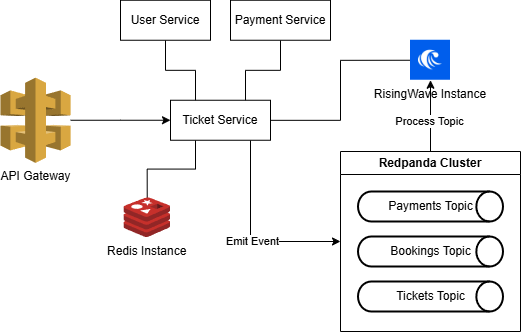
\includegraphics[width=0.8\textwidth]{resources/chapter-3/architecture-event-driven.png}
  \caption{\textit{Event-Driven Architecture}}
  \label{fig:solution-event-driven-architecture}
\end{figure}

\textit{Instance} Redpanda dapat dengan mudah dibuat \textit{cluster} dan \textit{partitioning}. Bila perlu, Redis dapat dikonfigurasikan dengan mode \textit{cluster} untuk \textit{redundancy} dan mode AOF untuk \textit{persistence}. Layanan lain seperti \textit{ticketing service} dan layanan pengguna dapat dengan mudah di-\textit{scale} dengan menambah jumlah \textit{instance}. Selain itu, RisingWave merupakan \textit{streaming database} yang \textit{cloud-native} sehingga dapat di-\textit{scale out} dengan mudah untuk meningkatkan \textit{throughput}.


% \bgroup
% \begin{table}[ht]
%   \def\arraystretch{1.3}
%   \caption{Perbandingan Ketiga Alternatif Solusi}
%   \label{tab:perbandingan-analisis-solusi}
%   \centering
%   \begin{tabular}{|p{2cm}|p{2cm}|p{2cm}|p{1.8cm}|p{1.7cm}|p{1.7cm}|}
%     \hline
%     Solusi           & Berjalan di berbagai perangkat                            & Melakukan \textit{targeted deployment} & Berjalan pada perangkat dengan sumber daya terbatas & Mengatur banyak perangkat & Waktu pembuatan sistem \\
%     \hline
%     Kubernetes       & Ya, seluruh perangkat yang dapat melakukan kontainerisasi & Ya                                     & Ya dengan K3s                                       & Ya                        & Cepat                  \\
%     \hline
%     Zookeper         & Ya, seluruh perangkat yang memiliki java                  & Tidak                                  & Tidak                                               & Ya                        & Cepat                  \\
%     \hline
%     LEONORE \& DIANE & Tidak                                                     & Tidak                                  & Mungkin                                             & Ya                        & Lama                   \\
%     \hline
%   \end{tabular}
% \end{table}
% \egroup